% !TEX root = ../SYSprojektrapport.tex
% SKAL STÅ I TOPPEN AF ALLE FILER FOR AT MASTER-filen KOMPILERES 

\label{Spaendingsstabilitet}

Spændingsstabilitet er et systems evne til at opretholde den nominelle spænding ved busbarere og forbrugere ved normale og unormale forhold i nettet. Spændingen ved belastning må maksimalt svinge med $\pm$10\% iht. INDSÆT STANDARD!, det er derfor vigtig at systemet kan regulere spændingen.  

Spændingsstabilitet er iht. figur \ref{fig:Overview} opdelt i \textit{Large- and Small Disturbance Voltage Stability} og herefter \textit{Short Term} og \textit{Long Term}. Store og små forstyrrelser henviser til hvor omfattende problemet er. \\
\textit{Small Disturbance Voltage Stability} kan være resultatet af et øgede forbrug samtidig med at en linje er ude pga. service, så der vil være et større tab i de resterende linjer, eller hvis en enkelt linje ryger ud pga. en fejl.\\
\textit{Large Disturbance Voltage Stability} er som regel resultatet af flere hændelser i nettet der skaber et spændingsfald i et større område eller i værste fald forårsager blackout.

Begge dele kan være \textit{Short Term} og \textit{Long Term}. Det kommer an på hvor hurtigt systemet kan reguleres, omlægges eller fjerne fejlen i nettet. På figur \ref{fig:VoltageTime} ses hvilke elementer der kan stabilisere systemet på kort og lang sigt. Til hurtigt regulering kan anvendes mindre generatorer, konverterer eller kondensator banke, hvor der over længere tid f.eks. kan laves en regulering i et kraftværker eller opstartes en gas turbine.  

\begin{figure}[H] % (alternativt [H])
	\centering
	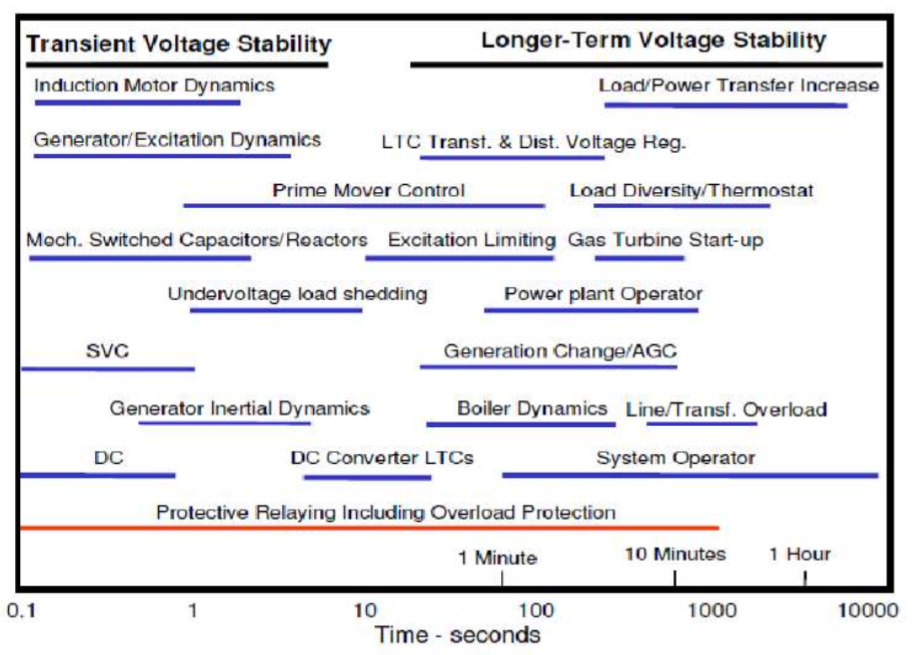
\includegraphics[width=0.6\textwidth]{figurer/Voltage_time}
	\caption{Oversigt over Short and Long Term disturbances}
	\label{fig:VoltageTime}
\end{figure}

Hovedsageligt opstår spændingsustabilitet når systemet ikke kan levere nok reaktiv effekt. Når der tilføjes reaktiv effekt skal spændingen stige, men hvis spændingen falder er systemet ustabilt. Spændingsustabilitet kan både forekomme som overspænding og spændingsfald. Overspænding kan ske ved for stor produktion i forhold til belastning, men også hvis der bliver tilføjet for meget reaktiv effekt i systemet pga. for meget kapacitiv belastning fra f.eks. shunt kondensatorer. 

Den største årsag til spændingsustabilitet er spændingsfald der hovedsageligt opstår pga. den induktive reaktans i transmissionslinjer. Tabet i linjerne forøges sammen med belastning, hvilket vil kræve en større mængde reaktiv effekt af systemet. På figur \ref{fig:Voltage1} ses et simpelt system med spændingskilde $E_{s}$, kabel impedans $Z_{LN}$, belastnings impedans $Z_{LD}$. 


\begin{figure}[H] % (alternativt [H])
	\centering
	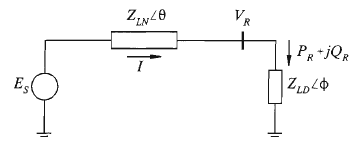
\includegraphics[width=0.5\textwidth]{figurer/Voltage_system}
	\caption{Skematisk diagram af et net system med forsyning, transmissionslinje og belastning}
	\label{fig:Voltage1}
\end{figure}

Ved at undersøge systemet med en variable belastning ses det at den maksimale effekt overførelse er hvor spændingen ved belastningen $V_{R}$ er lig med spændingsfaldet i transmissionslinjen. Dette kaldes det kritiske punkt. Det er også i dette punkt hvor $Z_{LN}$ og $Z_{LD}$ er lige store. Hvis $Z_{LD}$ er mindre end $Z_{LN}$ stiger strømmen og spændingen bliver mindre, det vil skabe et stort spændingsfald og gøre systemet ustabilt. Det normale arbejdspunkt i et system ligger på ca 80\% af maks. belastningen.

\begin{figure}[H] % (alternativt [H])
	\centering
	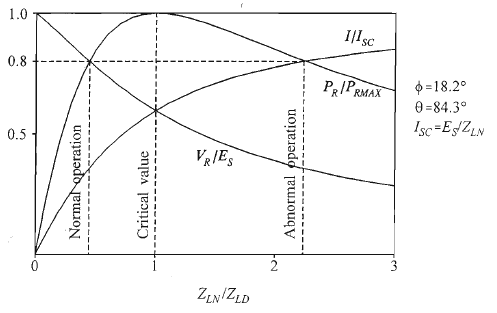
\includegraphics[width=0.7\textwidth]{figurer/Voltage_curve}
	\caption{graf for variable belastning i systemet}
	\label{fig:Voltage2}
\end{figure}


\section{Batterier som aktiv netelement}

Da batterier er en fleksibel belastning kan de hjælpe på spændingsstabilitet, både ved overspænding og spændingsfald. Ved normal drift stabiliseres nettet da batterier kan af- og oplades alt efter hvor hårdt nettet er belastet. Ved service af kabler og andet udstyr kan batterier aflaste det resterende net så det ikke belastes så hårdt og ved pludselig fejl kan batterierne hurtigt kobles ind, indtil der bliver omlagt forbindelser i understationerne. Batterierne kan derfor blive en stor hjælp for spændingsstabilitet og kan hjælpe på små og store forstyrrelser og på kort og lang sigt.